\documentclass[runningheads]{llncs}
\usepackage[T1]{fontenc}
\usepackage{graphicx}
\usepackage{color}
\usepackage{amsmath}

%\renewcommand\UrlFont{\color{blue}\rmfamily}
%\urlstyle{rm}
%
\begin{document}
%
\title{Conditional Variational Autoencoders with Fuzzy Inference}
\titlerunning{CVAE Fuzzy Inference}
%
\author{Yury Gurov\inst{1}\orcidID{0000-0002-7033-9996} \and
Danil Khilkov\inst{1}\orcidID{0000-0001-9284-6924}}
\authorrunning{Y. Gurov and D. Khilkov}
%
\institute{NIIAS Institute of Informatization, Automation and Communication in Railway Transport, Russia, Moscow
109029 Nizhegorodskaya str., 27 bldg. 1
\email{info@vniias.ru}\\
\url{www.vniias.ru/} 
}
%
\maketitle              % typeset the header of the contribution
%
\begin{abstract}
We present an approach to constructing Conditional Variational Autoencoders (C-VAE) models with fuzzy inference during classification.
This preserves disentangling capabilities of VAE and at the same time performs latent space clusterization.
Fuzzy C-VAE model provides useful features for anomaly detection, utilizing partially labeled datasets and controlled generation of new samples.
%
\keywords{fuzzy logic  \and deep learning \and fuzzy inference \and Conditional Variational Autoencoders \and fuzzy cvae \and neuro-fuzzy}
\end{abstract}
%
%
%
\section{Introduction}

Hybrid neuro-fuzzy systems has a long time history and is still an active research area \cite{DECAMPOSSOUZA2020106275}.
Main feature that attract attemtion to neuro-fuzzy systems is possibility to combine the power of neural network with advantages of fuzzy logic, such a human-like reasoning.
At this work we propose an approach to constructing Conditional Variational Autoencoders (C-VAE) \cite{kingma2022autoencoding,Kingma_2019,SohnCVAE} models with fuzzy inference during classification phase.
This approach may preserve disentangling capabilities of VAE and at the same time performs latent space clusterization.
Such fuzzy C-VAE model provides useful features for anomaly detection, utilization of partially labeled datasets and controlled generation of new samples.

The source code is available at GitHub repository\footnote{https://github.com/kenoma/pytorch-fuzzy}.

\section{Related work}

In~\cite{Bolat2020} attempt to apply fuzzy logic to the latent space of VAE was made with fuzzy c-mean clustering.
Main drawback of this approach is that it requires prior knowledge about problem domain number of clusters and their iterpretations.



In~\cite{RAMCHANDRAN2024110113} conditional VAE was modified in a way to process partially observed datasets. 
Authors proposed method that augments the conditional VAEs with a prior distribution for the missing covariates and estimates their posterior using amortised variational inference.
At first sigh this approach has nothing to do with fuzzy logic, but it provides insigh into the problem of latent space clustering.



\section{Methods}

\subsection{Variational Autoencoders}
Variational inference is used to approximate a posterior distribution of a directed graphical model whose latent variables and parameters are intractable.
The Variational Auto-Encoder (VAE) combines this approach with an autoencoder framework to learn the prior distribution of a latent space, $p_\theta(z)$, with parameters $\theta$.
The idea is that the prior distribution can then be sampled to produce a latent code, $z$, which is passed as input to the decoder to produce a sample output, $\tilde{x}$. 
VAEs consists of two NN for the probabilistic encoding and decoding process (see Figure 1a). 
As the true underlying distribution of the posterior is intractable and complex, a simple parametric surrogate distribution, $q_\Phi(z|x)$ (such as a Gaussian), with parameters $\Phi$, is assumed to approximate the distribution and is optimized for best fit. 
The encoder network implicitly models the surrogate distribution, by mapping the distribution parameters, $\Phi$, during the training process. 
The resulting model, $q_\Phi(z|x)$, is referred to as the recognition model. 
The optimization process of the recognition model revolves around minimizing the Kullback-Leibler (KL) divergence between the posterior and surrogate distributions.
Once the latent prior distribution is learned, $z$ can be sampled via the reparameterization trick.
The (probabilistic) decoder network performs a mapping of the latent code to a structured sample output for each sample, thus producing a distribution of outputs, $p_\theta (x|z)$.

\subsection{Conditional VAE}
The C-VAE expands upon the framework of the VAE, by combining variational inference with a conditional directed graphical model. 
In the case of C-VAE, the objective is to learn a prior distribution of the latent space that is conditioned on an input variable $y$ such that $p_\theta (z|y)$ (see Fig. \ref{fig:overview}b).
The conditioning of the distributions results in a prior that is modulated, by the input variable, creating a method to control modality of the output. 

\begin{figure}
    \centering
    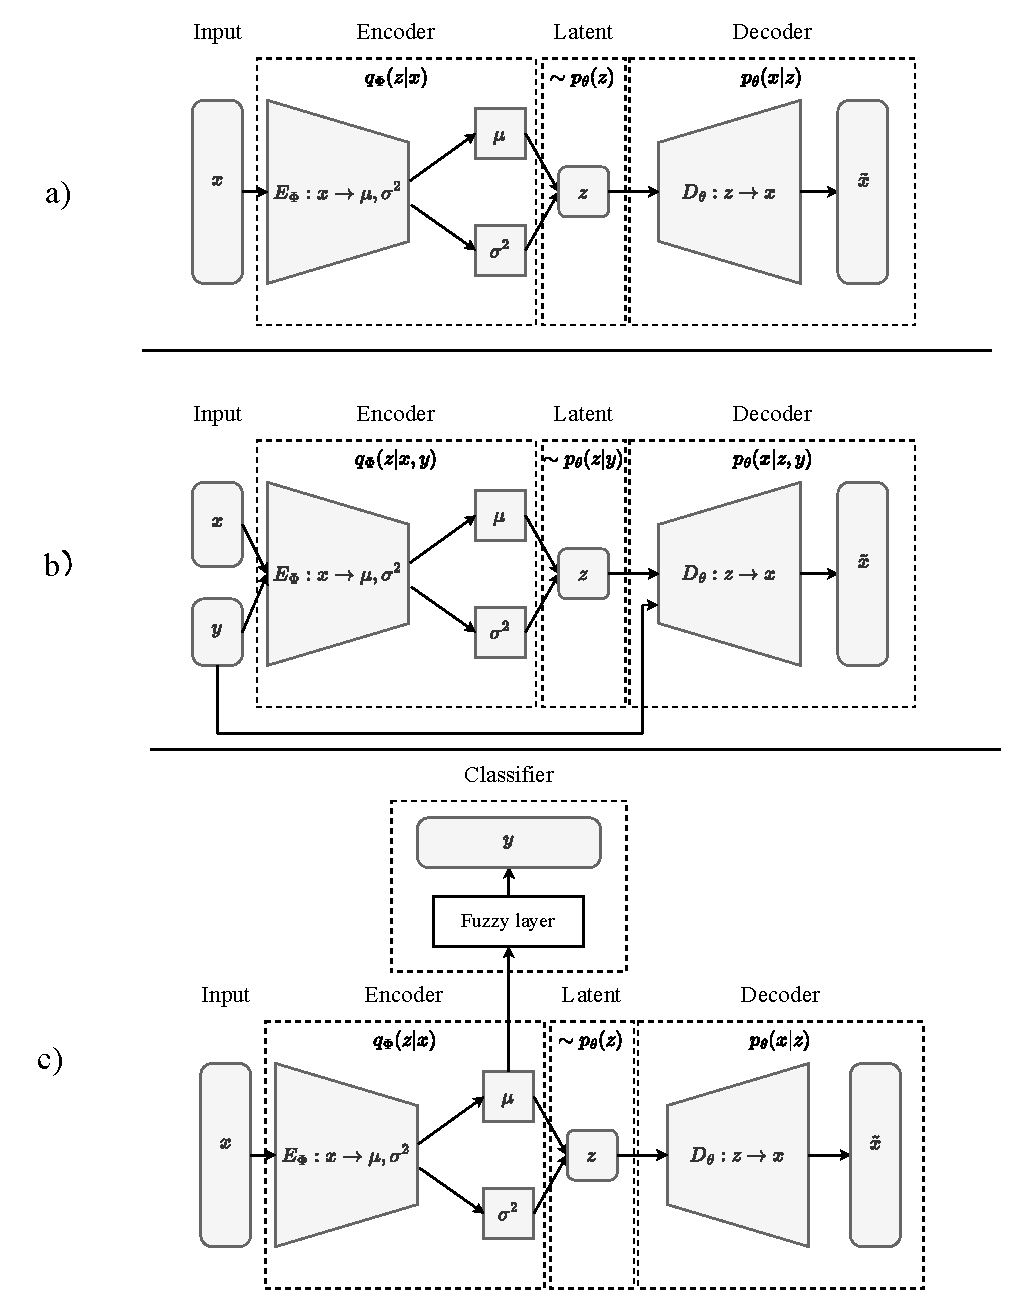
\includegraphics[width=0.8\textwidth]{fig_1.pdf}
    \caption{Overview of the $a)$ VAE $b)$ CVAE by~\cite{SohnCVAE} and $c)$ proposed fuzzy C-VAE model.}
    \label{fig:overview}
\end{figure}

\subsection{Fuzzy C-VAE}

We propose C-VAE architecture where additional conditions are applied only to $/mu$ component in order to reorganize the latent space structure (see Fig\ref{fig:overview}c).
Reorganization achieved by using fuzzy term functions, where each term associated with sole condition i.e. label.
Multidimentional Gaussian function is used to represent the fuzzy term function:

\[ 
   \nu(z, A_i) = e^{|| [A_i . \tilde{z}]_{1 \cdots m} ||^2},
\]
where $m$ is a latent space dimension size, $i$ denotes term number, $\tilde{z} = [z_1, z_2, \cdots, z_m, 1]$ and $A_i$ is transformation matrix in form 

\[ 
    A_{(m+1) \times (m+1)}= 
    \begin{bmatrix}
        s_{1} & a_{12} & \cdots & a_{1m} & c_{1}\\
        a_{21} & s_{2} & \cdots & a_{2m} & c_{2}\\
        \vdots & \vdots & \ddots & \vdots & c_{3}\\
        a_{m1} & a_{m2} & \cdots & s_{m} & c_{m}\\
        0 & 0 & \cdots & 0 & 1
    \end{bmatrix},
\]
with $c_{1\cdots m}$ centroid position, $s_{1\cdots m}$ scaling factor and $a_{1\cdots m, 1\cdots m}$ as alignment coefficients.
Such representation of multidimentional Gaussian term function easyly can be adopted for use in any modern machine learning framework.
Set of $\nu(z, A_i)$ we call a fuzzy layer.
Intuition behind fuzzy layer is that during training procedure every input vector $z$ will be forced to group closer near centroid of correspoinding term function.
Disentangling features of VAE combined with clustering possibilities of fuzzy layer provides a way to learn suprvised latent space which can be useful for anomaly detection and other tasks we discuss further.

\subsection{Learning Fuzzy C-VAE}

To train fuzzy C-VAE we use the same loss function as in standard VAE with addition of fuzzy layer loss:

\[
    Loss = MSE(\tilde{x}, x) + KL(\mu, \log{\sigma^2}) + FZ(\tilde{y}, y),
\]
where $MSE(\tilde{x}, x)$ is reconstruction loss, $KL(\mu, \log{\sigma^2})$ is the KL-divergence (for more details see~\cite{kingma2022autoencoding}) and $FZ(\tilde{y}, y)$ represents the mean squared error between the output and target conditional verctor.

Main drawback of fuzzy layer is that in hight dimensional cases it's hard to find good initial values for centroids and scaling factors mainly due to vanishing gradients.
Is such a case it is possible to pass to fuzzy layer subsection of vector $/mu$ leaving remained part to be trained by VAE without any conditional restrictions. 


\section{Experiments}

In this paper we would like to demonstrate ideas of fuzzy C-VAE on playground MNIST dataset.
To make demostration fancy we provide additional label to samples of MNIST dataset.
This label separates numbers with closed round loops in outline $0,6,8,9$ from numbers without it $1,2,3,4,5,7$.
To make reasonable reconstruction loss we set size of the latent vector equal to 12 but only 2 first values of this vector are passed to fuzzy layer.
The fuzzy CVAE model is trained using the Adam optimizer~\cite{kingma2017adam}.

\subsection{Latent space clusterization}

On Figure~\ref{fig:vae-clustering} is depicted latent space structure resulted by vanila VAE without any conditional restrictions.
Despite the fact that points in VAE latent space are grouped in clusters corresponding to each number this structure has very complex topology.
Without application of prior knowledge about number labels task of extracting corresponding clusters is very challenging.

Passing label information directly to fuzzy C-VAE during training leads to fine grained latent space structure as shown on Figure \ref{fig:vae-clustering}.
First two components of latent vector on which fuzzy layer is applied have formed clusters corresponding to each number.
Meanwhile remained components of latent vector preserves complex topology like pure VAE.
Reconstruction losses for VAE and fuzzy C-VAE during our experiments were almost the same while KL-loss for fuzzy C-VAE was slightly highter all the time.
Classification accuracy of fuzzy C-VAE depends on many factors of network topology and training scenario but limit of 99\% is easily achieved.
Figure~\ref{fig:fcvae-classes} shows how fuzzy C-VAE is able to classify samples.

\begin{figure}
    \centering
    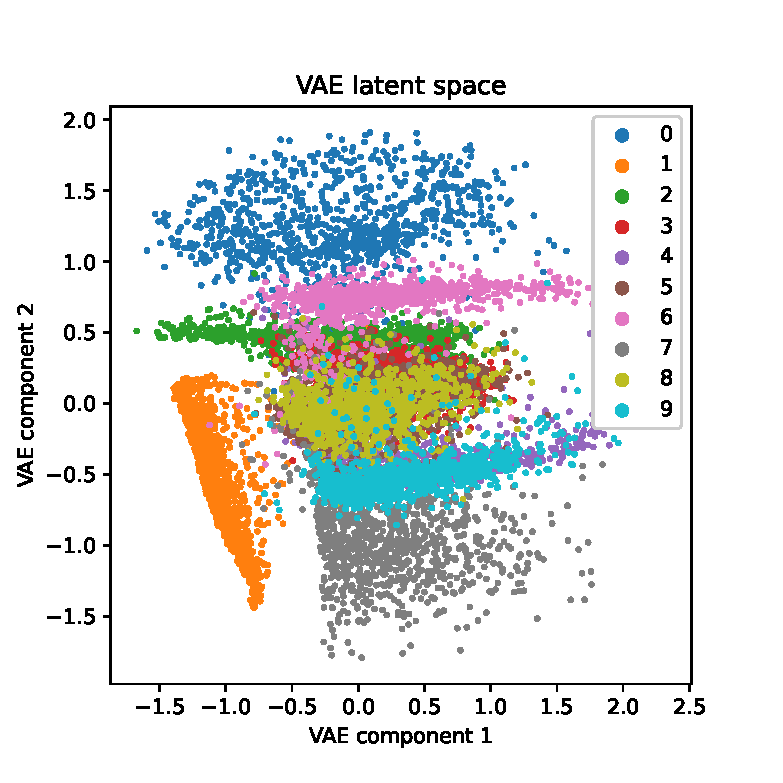
\includegraphics[width=1\textwidth]{fig2a-vae-all-features.eps}
    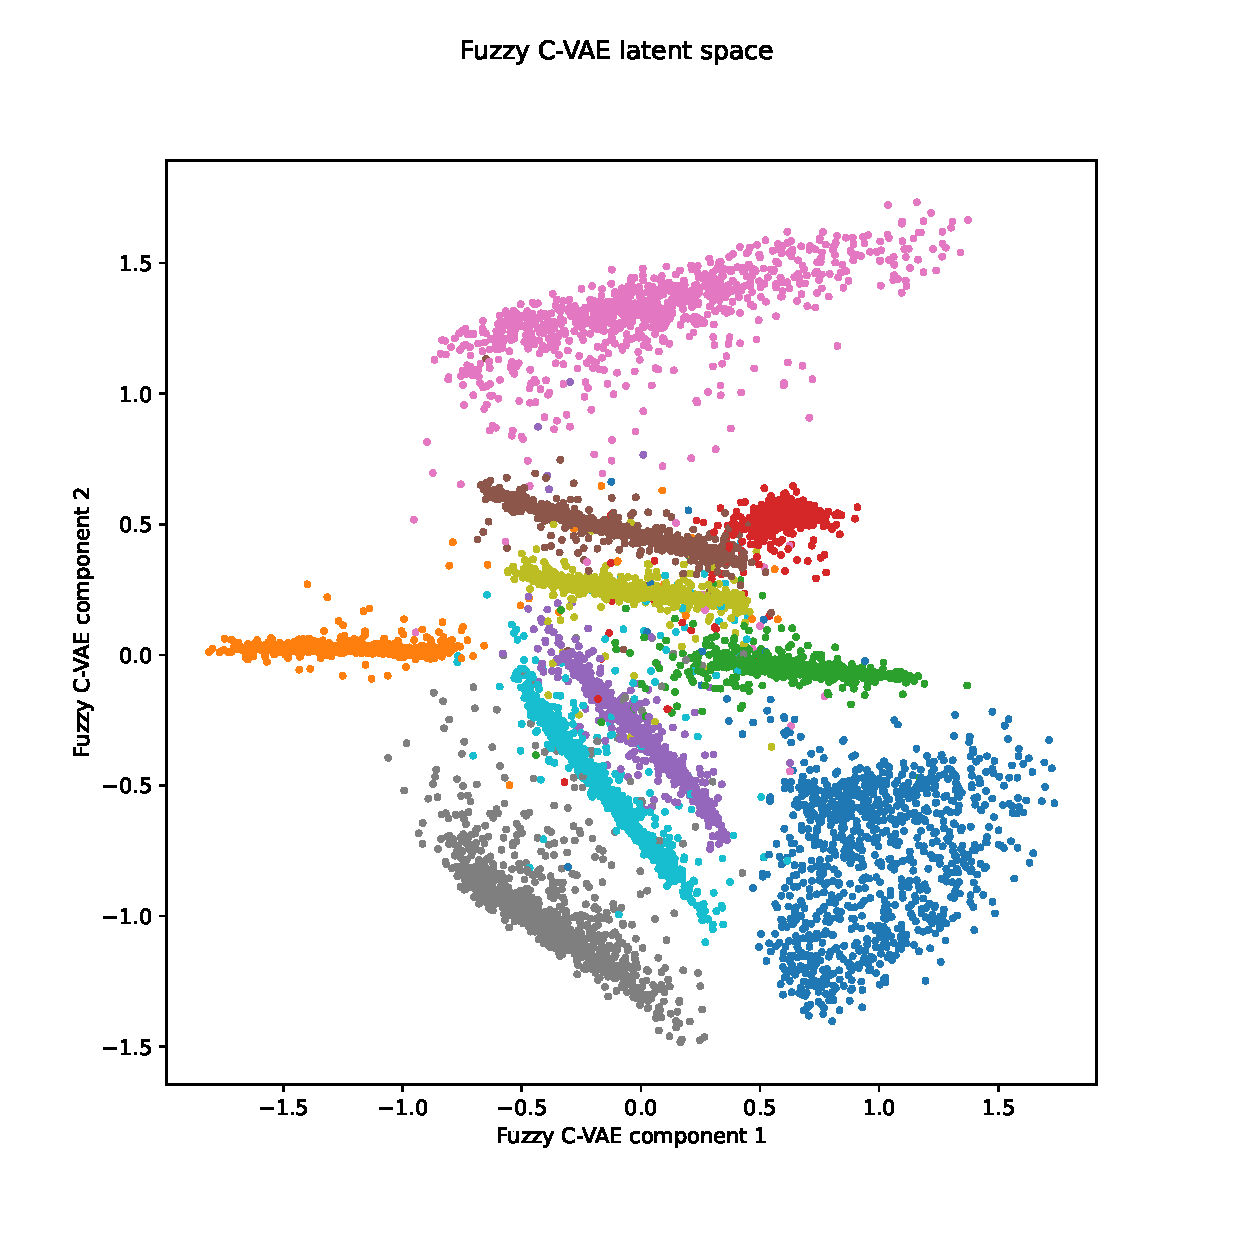
\includegraphics[width=1\textwidth]{fig2b-fcvae-all-features.eps}
    
    \caption{Latent space granulation for vanila VAE (top) and Fuzzy C-VAE (bottom)}
    \label{fig:clustering}
\end{figure}

\begin{figure}
    \centering
    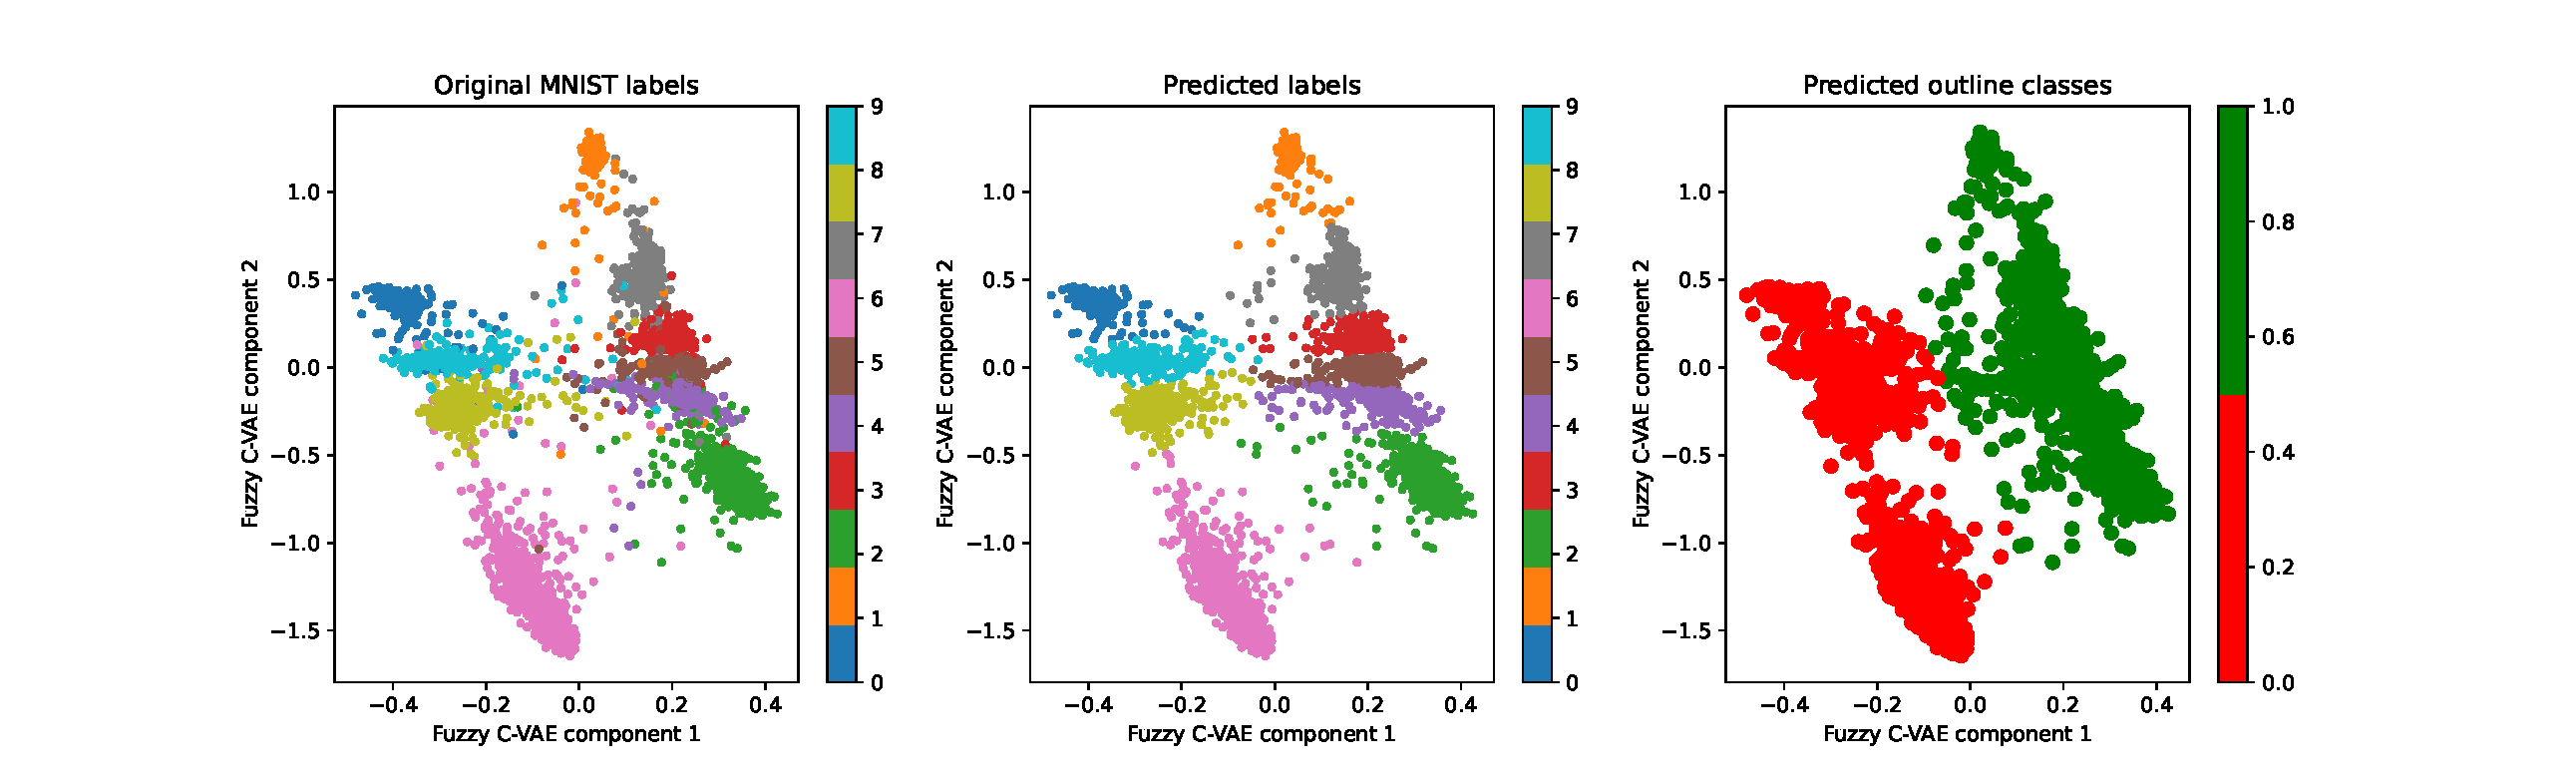
\includegraphics[width=1\textwidth]{fig3-fcvae-classification.eps}
    \caption{Fuzzy C-VAE latent space colored by true number labels (left) predicted number labels (center) and predicted outline class (right) }
    \label{fig:fcvae-classes}
\end{figure}

\subsection{Controlled samples generation}

After training procedure it is possible extract from matrices $A_i$ cluster characteristics such a centroids, scaling and aligment factors to understand latent space structure.
Thats make possible use fuzzy C-VAE for sample generation with predefined characteristics as shown on Figure \ref{fig:samples-generation}.

\begin{figure} 
    \centering
    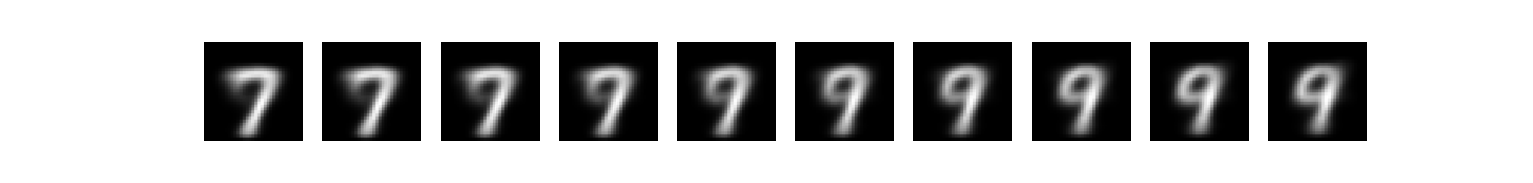
\includegraphics[width=1\textwidth]{fig4-sample-generation.eps}
    \caption{Fuzzy C-VAE latent space colored by true number labels (left) predicted number labels (center) and predicted outline class (right) }
    \label{fig:samples-generation}
\end{figure}

\subsection{Anomaly detection}

Fuzzy C-VAE provides convinient way to design anomaly detection model.
In a natural way every single term with underlying Gaussian distribution can provide mechanism to detect anomaly. 

To demonstrate anomaly detection on MNIST we use EMNIST dataset~\cite{cohenafshartapsonschaik2017} with letters subset.
Anomaly rate can be defined as 
\[
    r_{a} = \max_i \nu(z_{a}, A_i),
\] 
where $z_{a}$ is latent vector for an sample.
Latent space for fuzzy C-VAE model was set to 12.

In Table \ref{table-anomaly} we provide statistics for $r_{a}$ for letter which were never passed through fuzzy C-VAE model during training phase.

\begin{table}[h!]
    \centering
    \begin{tabular}{lr}
        Symbols & Detected anomaly rate \\
        0123456789 & 0.18 \\
        Oo & 0.36 \\
        Ww & 0.39 \\
        Nn & 0.61 \\
        Mm & 0.62 \\
        Ii & 0.63 \\
        Ff & 0.65 \\
        Vv & 0.66 \\
        Uu & 0.69 \\
        Ll & 0.70 \\
        Aa & 0.71 \\
        Pp & 0.71 \\
        Tt & 0.73 \\
        Dd & 0.75 \\
        Gg & 0.76 \\
        Qq & 0.76 \\
        Yy & 0.78 \\
        Bb & 0.79 \\
        Kk & 0.79 \\
        Cc & 0.80 \\
        Hh & 0.81 \\
        Ee & 0.82 \\
        Ss & 0.82 \\
        Rr & 0.83 \\
        Jj & 0.85 \\
        Zz & 0.86 \\
        Xx & 0.89 \\
    \end{tabular}        
    \caption{Anomaly rate for symbols from MNIST and EMNIST datasets}
    \label{table-anomaly}
\end{table}



\subsection{Learning on partially labeled dataset}

Structure of fuzzy C-VAE model allows to pass unlabeled data sample to update only VAE weight.
This feature can be useful with training on dataset with limited expert knowledge in order to make VAE part of model more reliable.
To achieve this loss function has to be modified
\[
    Loss = MSE(\tilde{x}, x) + KL(\mu, \log{\sigma^2}) + \gamma * L(x, \tilde{y}, y),
\]
where $\gamma > 1$ is a hyperparameter that controls the influence of fuzzy part of model and
\[
    L(x, \tilde{y}, y) = \begin{cases}
        0,&~x~\mbox{is~unlabeled}\\
        FZ(\tilde{y}, y),&~x~\mbox{is~labeled}
      \end{cases}.
\]

On Fugure~\ref{fig:accuracy-vs-unlabeled-rate} we provide model performance on MNIST dataset with different unlabeled rate.

\begin{figure}[h]  
    \centering
    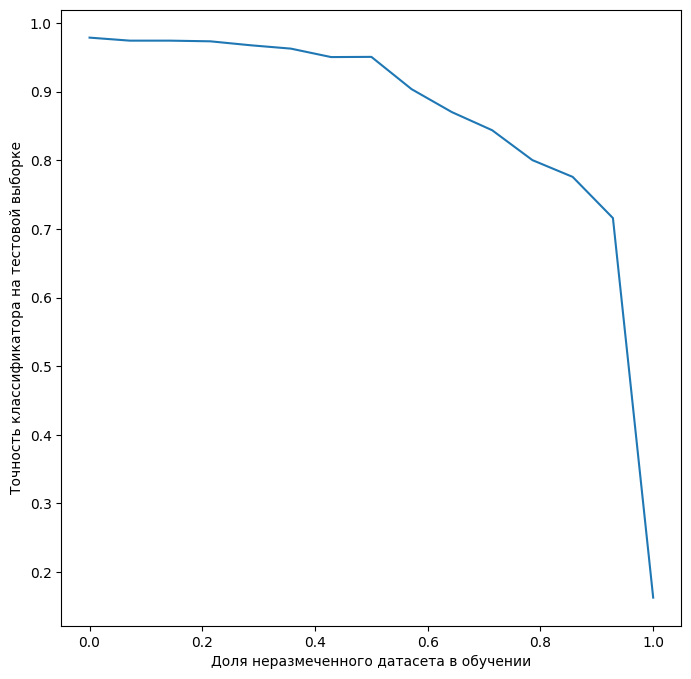
\includegraphics[width=1\textwidth]{fig5-accuracy-vs-unlabeled-rate.png}
    \caption{ Model test set accuracy on MNIST dataset with different unlabeled rate. }\label{fig:accuracy-vs-unlabeled-rate}
\end{figure}

With this results we can conclude that it's reasonable to pass unlabeled samples during trainig to maintain better reconstruction quality.
On the other side presented technique may be useful during markup phase to determine while dataset sufficiently labeled and further markup is not useful

\section{Discussion}

In this paper, we introduced a novel fuzzy inference layer to improve the performance of conditional VAEs. 
We achieve this by making trainable multidimentional representation of fuzzy term.
The method that we proposed is applicable to a variety of conditional VAE models. 
The efficacy of our proposed method was demonstrated on MNIST dataset. 
Whereas fuzzy conditions influence on VAE should be discussed more deeply we leave it for future work. 

\bibliographystyle{splncs04}
\bibliography{refs.bib}

\end{document}
